% Chapter Template

\chapter{Análisis de tipos de entrada}

\label{Chapter2} % Change X to a consecutive number; for referencing this chapter elsewhere, use \ref{ChapterX}

%----------------------------------------------------------------------------------------

\section{MathML}


\subsection{¿Qué es MathML?}

MathML (Mathematical Markup Language) \cite{2} es un dialecto XML para describir notaciones matemáticas que busca capturar tanto la estructura
como el contenido. Su objetivo es integrar las fórmulas matemáticas en las páginas de Internet y otros documentos.
Forma parte de HTML5 y de un estándar ISO ISO/IEC DIS 40314 desde el año 2015.

Una de las ventajas de MathML es que es un estándar de representación de fórmulas matemáticas para la World Wide Web (W3) y los principales y más usados
navegadores de Internet tienen integrado de manera nativa el soporte para éste tipo de contenido haciéndolo una aplicación accesible.

MathML consiste de un número de tags XML que pueden ser usados
para el marcado de una ecuación en términos de su representación y su semántica. Ésto último es sumamente importante
ya que MathML busca capturar el significado detrás de la ecuación además de concentrarse en cómo ésta será formateada y mostrada en pantalla.

MathML busca facilitar el uso y el re uso de contenido científico en la Web. La versatilidad de éste lenguaje de marcado nos permite aprovechar
su notación para displays visuales de alta calidad y su contenido para aplicaciones más semánticas cómo software científico o sintetizadores de voz.

Como se mencionó MathML codifica tanto la estructura como el contenido de las expresiones matemáticas.
A través del marcado de presentación (Presentation MathML o PMathML) se pueden desplegar expresiones matemáticas, y mediante el marcado de contenido
(Content MathML o CMathML) se puede representar el significado de las expresiones matemáticas.

\subsection{PMathML}

El \textbf{marcado de presentación} tiene como objetivo principal describir la estructura de una fórmula matemática.
Los elementos de presentación corresponden a los \textbf{constructores} de la notación matemática tradicional, en la última versión de MathML se incluyen
37 tags que pueden ser usados para representar una fórmula matemática. Los tags más usados son \textit{<mi>, <mo>, <mrow>} para indicar una \textit{variables, operadores,
expresiones anidadas}, respectivamente.

\subsection{CMathML}

El \textbf{marcado de contenido} tiene como objetivo principal describir la semántica de una fórmula matemática.
Provee una lista mucho más amplia de tags para ser usados con respecto a PMathML, sumando un total de 129.
Entre los tags más usados tenemos <apply>, <ci>, <cn>. El primero de ellos se utiliza para hacer explícita la aplicación de un
operador a sus children's (tags hijos), dejando en claro cuál es el scope de aplicación. El segundo tag se utiliza para describir variables y el tercero
de ellos se utiliza para describir los números. CMathML contiene un tag en específico para cada operación matemática, lo que lo hace más específico que PMathML
ya que PMathML contiene un tag solo para algunas operaciones (como la suma o multiplicación).

En la siguiente figura se puede observar cómo se describe en PMathML y CMathML para la siguiente fórmula matemática: $x + \frac{a}{b}$

\begin{figure}[H]
\centering
  \begin{minipage}[b]{0.4\textwidth}
    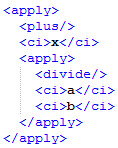
\includegraphics{Figures/ejemplo_cmathml}
    \caption[]{CMathML}
  \end{minipage}
  \begin{minipage}[b]{0.4\textwidth}
    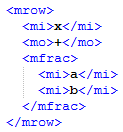
\includegraphics{Figures/ejemplo_pmathml}
    \caption[]{PMathML}
  \end{minipage}
\label{fig:ejemplo_cmathml}
\end{figure}

\subsection{¿Por qué CMathML?}
Hay ciertas expresiones matemáticas que pueden tener distintas interpretaciones, esto la hace una expresión ambigua, ya que muchas veces
depende del contexto su correcta interpretación. Supongamos la siguiente fórmula matemática:
$$f^{-1}$$
Que puede interpretarse como la función inversa de f o, también como, la variable f elevado a -1. Para ello veamos cómo es su marcado tanto en PMathML como en CMathML.
Para PMathML tenemos el siguiente XML:
\lstset{language=XML}
\begin{lstlisting}
<math xmlns="http://www.w3.org/1998/Math/MathML">
  <msup>
    <mi>f</mi>
    <mn>-1</mn>
  </msup>
</math>
\end{lstlisting}

Podemos ver que, dado que PMathML intenta solo capturar su presentación, su XML asociado sigue siendo ambiguo. Ya que la etiqueta \textit{<msup>} solo
señala que -1 es el superíndice de f. Lo que lo vuelve ambiguo tal como se escribe su expresión matemática.

En cambio para CMathML, ya que ésta intenta capturar su semántica, podemos ver que tenemos dos posibles XML asociados a esta fórmula matemática.

\lstset{language=XML}
\begin{lstlisting}
<math xmlns="http://www.w3.org/1998/Math/MathML">
  <apply>
    <inverse/>
    <ci type="function">f</ci>
  </apply>
</math>
\end{lstlisting}

y también tenemos

\lstset{language=XML}
\begin{lstlisting}
<math xmlns="http://www.w3.org/1998/Math/MathML">
  <apply>
    <power/>
    <ci type="function">f</ci>
    <cn>-1</cn>
  </apply>
</math>
\end{lstlisting}

Podemos ver que para CMathML queda claro de qué interpretación queremos asociar al XML. Ya que en el primer caso tenemos el tag \textit{<inverse>}
aplicado a la variable \textit{f} que habla de la inversa de f. Y en el segundo tenemos el tag \textit{<power>} que denota el exponente \textit{-1} aplicado a \textit{f}.

Otra ventaja que tiene CMathML sobre PMathML es que existen herramientas para hacer el pasaje de CMathML a PMathML, pero debido a la ambiguedad de PMathML no existe una herramienta que lo haga en la otra dirección.

Esta es la razón principal que CMathML es el adecuado para la PoC que acompaña este trabajo final, es el lenguaje de marcado
que más se acerca a la lectura en lenguaje natural.

\section{\LaTeX}

\subsection{¿Qué es \LaTeX ?}

Según Wikipedia, \LaTeX\ es un sistema de composición de textos, orientado a la creación de documentos escritos que
presenten una alta calidad tipográfica. Por sus características y posibilidades, es usado de forma especialmente intensa en la
generación de artículos y libros científicos que incluyen, entre otros elementos, expresiones matemáticas.

Lo cierto es que \LaTeX posee a su disposición muchos paquetes para ser importados que hacen más fácil la escritura de
expresiones matemáticas. Cualquier expresión matemática puede ser escrita usando \LaTeX.

Latex fue diseñado específicamente para ser escrito por humanos por eso éste sistema es el más usado para la generación de archivos científicos y, por lo tanto, muchas expresiones matemáticas
son escritas con \LaTeX, lo que hace que \LaTeX sea el lenguaje más usado para escribir éste tipo de expresiones.
Si bien MathML es usado por distintos softwares científicos y navegadores web, no es realmente el lenguaje más usado para escribir expresiones matemáticas desde
el lado del usuario, como lo es \LaTeX.

Esta es la razón por la que \LaTeX es considerado como un tipo de entrada válido para la PoC.

A modo ilustrativo, veamos cómo es en sintaxis \LaTeX la fórmula $x + \frac{a}{b}$:

\verb|$x + \frac{a}{b}$|

Podemos notar que, al igual que CMathML, captura la estructura y el contenido de la expresión. Sabiendo que \verb|\frac| es la manera de escribir una fracción y con \textit{+} podemos escrbir la suma, podemos leer con facilidad la expresión matemática mencionada y darle el respectivo significado. Cabe mencionar, que hay una relación entre CMathML y \LaTeX y será explicado más adelante en este documento.

\LaTeX además de ser usado ampliamente por científicos para escribir sus publicaciones y documentos, también es usado para describir
algunas expresiones matemáticas en Internet. Tal es así el caso de Wikipedia, que para cada fórmula matemática que tenga presente en algún artículo en línea posee dentro de el atributo \textit{alt} del tag \textit{<img>}
su descripción en lenguaje \LaTeX.

Por ejemplo, veamos en el artículo que explica las ecuaciones de segundo grado %(Cita: https: es.wikipedia.org wiki Ecuación_de_segundo_grado) en su segunda figura tenemos
$$x = \frac{-b \pm \sqrt {b^2-4ac}}{2a}$$

mientras que su código HTML tenemos
\\
\verb|<img|\\
\verb|  class="tex" src="expresion.png"|\\
\verb|  alt="x = \frac{-b \pm \sqrt {b^2-4ac}}{2a}"|\\
\verb|>|

\subsection{Análisis de \LaTeX y MathML}

Si bien la relación entre Latex y CMathML\cite{5} es muy sensible y fina, existe. Comencemos diferenciado estas tecnologías desde un punto de vista de usabilidad y comprensión, así también desde tipo de entrada.

\begin{itemize}
\item \textbf{Usabilidad}: Latex es el lenguaje más usado para escribir documentos y artículos científicos, hay tutoriales y documentación con ejemplos para aprender a escribir usando este lenguaje. Latex funciona desde el lado del usuario (\textit{user-side}), mientras que MathML es la aplicación más usada para renderizar expresiones matemáticas en distintos softwares, y funciona desde el lado del servidor (\textit{server-side}). En muchos artículos se menciona que MathML es la representación que las computadoras entienden de las expresiones que conocemos.
\item \textbf{Compresión desde el usuario}: Una expresión matemática, tanto escrita con Latex o MathML, pueden ser leídas con el mismo grado de dificultad. Si la expresión es más avanzada, la lectura desde un humano puede requerir un poco más de atención. Pero a la hora de la escritura, Latex es más amigable que MathML.
\item \textbf{Tipo de entrada}: MathML saca ventaja sobre Latex de ésto ya que, como se mencionó, MathML es un dialecto XML que nos permite renderizar cualquier expresión matemática y consigo trae todas las ventajas que tiene una aplicación XML. El parser es un componente estándar, por lo tanto no es necesario crear un parser específico para cada versión de lenguaje XML. Esto posibilita el empleo de cualquiera de los analizadores disponibles. De esta manera se evitan bugs y se acelera el desarrollo de aplicaciones. Pero no funciona así con Latex, debido que Latex es un lenguaje de programación y no un estándar puede ser extendido por lo tanto no hay un parser disponible para poder particionar una expresión latex para procesar partes más atómicas.
\end{itemize}

Las conclusiones hasta el momento es que Latex es el lenguaje más elegido por los usuarios y MathML es la aplicación más elegida para desarrollar el software. Es por eso que en ésta tesis se intenta hacer un ligamento entre estas tecnologías y aprovechar las ventajas de cada uno.